\documentclass{standalone}
\usepackage{tikz,tikz-3dplot}
\usetikzlibrary{perspective,patterns}
\usetikzlibrary{calc,fadings,decorations.pathreplacing}
\usetikzlibrary{shapes,fit}
\usetikzlibrary{hobby}
\usetikzlibrary{arrows.meta}
\begin{document}
\tikzset{illustration/.style={very thin}}
\tikzset{dimension/.style={very thin,lightgray}}
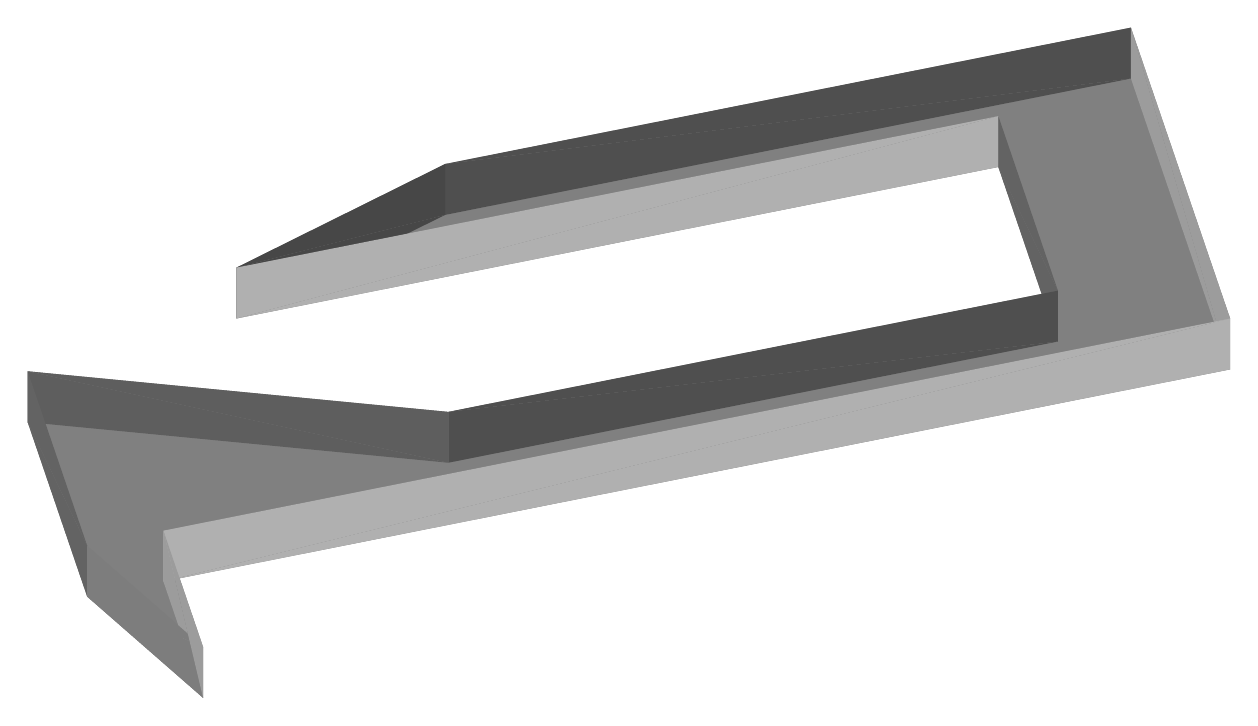
\begin{tikzpicture}[3d view={-14.598411358038462}{49.78019809531759},fill=gray]
\fill (1,0)--(1,2)--(15,2)--(15,7)--(6,7)--(3,6)--(13,6)--(13,3)--(5,3)--(0,5)--(0,2)--cycle;
\fill (1.0,0.0,1.0)--(1.0,2.0,1.0)--(15.0,2.0,1.0)--(15.0,7.0,1.0)--(6.0,7.0,1.0)--(3.0,6.0,1.0)--(13.0,6.0,1.0)--(13.0,3.0,1.0)--(5.0,3.0,1.0)--(0.0,5.0,1.0)--(0.0,2.0,1.0)--cycle;
\fill[white!31!black] (15,7,0)--(6.0,7.0,1.0)--(15.0,7.0,1.0)--cycle;
\fill[white!61!black] (15,2,0)--(15,7,0)--(15.0,7.0,1.0)--cycle;
\fill[white!31!black] (15,7,0)--(6,7,0)--(6.0,7.0,1.0)--cycle;
\fill[white!69!black] (3,6,0)--(13,6,0)--(13.0,6.0,1.0)--cycle;
\fill[white!39!black] (13,6,0)--(13.0,3.0,1.0)--(13.0,6.0,1.0)--cycle;
\fill[white!61!black] (15,2,0)--(15.0,7.0,1.0)--(15.0,2.0,1.0)--cycle;
\fill[white!39!black] (13,6,0)--(13,3,0)--(13.0,3.0,1.0)--cycle;
\fill[white!28!black] (6,7,0)--(3.0,6.0,1.0)--(6.0,7.0,1.0)--cycle;
\fill[white!28!black] (6,7,0)--(3,6,0)--(3.0,6.0,1.0)--cycle;
\fill[white!69!black] (3,6,0)--(13.0,6.0,1.0)--(3.0,6.0,1.0)--cycle;
\fill[white!31!black] (13,3,0)--(5.0,3.0,1.0)--(13.0,3.0,1.0)--cycle;
\fill[white!37!black] (5,3,0)--(0,5,0)--(0.0,5.0,1.0)--cycle;
\fill[white!31!black] (13,3,0)--(5,3,0)--(5.0,3.0,1.0)--cycle;
\fill[white!69!black] (1,2,0)--(15,2,0)--(15.0,2.0,1.0)--cycle;
\fill[white!37!black] (5,3,0)--(0.0,5.0,1.0)--(5.0,3.0,1.0)--cycle;
\fill[white!39!black] (0,5,0)--(0.0,2.0,1.0)--(0.0,5.0,1.0)--cycle;
\fill[white!39!black] (0,5,0)--(0,2,0)--(0.0,2.0,1.0)--cycle;
\fill[white!69!black] (1,2,0)--(15.0,2.0,1.0)--(1.0,2.0,1.0)--cycle;
\fill[white!61!black] (1,0,0)--(1,2,0)--(1.0,2.0,1.0)--cycle;
\fill[white!49!black] (0,2,0)--(1.0,0.0,1.0)--(0.0,2.0,1.0)--cycle;
\fill[white!49!black] (0,2,0)--(1,0,0)--(1.0,0.0,1.0)--cycle;
\fill[white!61!black] (1,0,0)--(1.0,2.0,1.0)--(1.0,0.0,1.0)--cycle;
\end{tikzpicture}
\end{document}
